%%% LaTeX Template: Article/Thesis/etc. with colored headings and special fonts
%%%
%%% Source: http://www.howtotex.com/
%%% Feel free to distribute this template, but please keep to referal to http://www.howtotex.com/ here.
%%% February 2011
%%%
%%% Last updated September 2018 by CDM

%%%  Preamble
\documentclass[11pt,letterpaper]{article}
\usepackage[margin=1.0in]{geometry}
\usepackage[T1]{fontenc}
\usepackage[bitstream-charter]{mathdesign}
\usepackage[latin1]{inputenc}					
\usepackage{amsmath}						
\usepackage{xcolor}
\usepackage{cite}
\usepackage{hyphenat}
\usepackage{graphicx}
\usepackage{float}
\usepackage{subfigure}
\usepackage{sectsty}
\usepackage[compact]{titlesec} 
\usepackage[tablegrid]{vhistory}
\allsectionsfont{\color{accentcolor}\scshape\selectfont}

%%% Definitions
\definecolor{accentcolor}{rgb}{0.0,0.0,0.5} 
\newcommand{\teamname}{Team Name}
\newcommand{\productname}{Product Name}
\newcommand{\coursename}{CSE 4316: Senior Design I}
\newcommand{\semester}{Fall 2020}
\newcommand{\docname}{Project Charter}
\newcommand{\department}{Department of Computer Science \& Engineering}
\newcommand{\university}{The University of Texas at Arlington}
\newcommand{\authors}{Alan Turing \\ Grace Hopper \\ John Von Neumann \\ Ada Lovelace \\ Charles Babbage}

%%% Headers and footers
\usepackage{fancyhdr}
	\pagestyle{fancy}						% Enabling the custom headers/footers
\usepackage{lastpage}	
	% Header (empty)
	\lhead{}
	\chead{}
	\rhead{}
	% Footer
	\lfoot{\footnotesize \teamname \ - \semester}
	\cfoot{}
	\rfoot{\footnotesize page \thepage\ of \pageref{LastPage}}	% "Page 1 of 2"
	\renewcommand{\headrulewidth}{0.0pt}
	\renewcommand{\footrulewidth}{0.4pt}

%%% Change the abstract environment
\usepackage[runin]{abstract}			% runin option for a run-in title
%\setlength\absleftindent{30pt}			% left margin
%\setlength\absrightindent{30pt}		% right margin
\abslabeldelim{\quad}	
\setlength{\abstitleskip}{-10pt}
\renewcommand{\abstractname}{}
\renewcommand{\abstracttextfont}{\color{accentcolor} \small \slshape}	% slanted text

%%% Start of the document
\begin{document}

%%% Cover sheet
{\centering \huge \color{accentcolor} \sc \textbf{\department \\ \university} \par}
\vspace{1 in}
{\centering \huge \color{accentcolor} \sc \textbf{\docname \\ \coursename \\ \semester} \par}
\vspace{0.5 in}
\begin{figure}[h!]
	\centering
   	
\includegraphics[width=0.60\textwidth]{images/test_image}
\end{figure}
\vspace{0.5 in}
{\centering \huge \color{accentcolor} \sc \textbf{\teamname \\ \productname} \par}
\vspace{0.5 in}
{\centering \large \sc \textbf{\authors} \par}
\newpage


%\vspace{1 in}
%\centerline{January 13th, 2012}
%\newpage

%%% Revision History
\begin{versionhistory}
  	\vhEntry{0.1}{10.01.2020}{GH}{document creation}
  	\vhEntry{0.2}{10.05.2020}{AT|GH}{complete draft}
  	\vhEntry{0.3}{10.12.2020}{AT|GH}{release candidate 1}
  	\vhEntry{1.0}{10.20.2020}{AT|GH|CB}{official release}
  	\vhEntry{1.1}{10.31.2020}{AL}{added customer change requests}
\end{versionhistory}
\newpage

%%% Table of contents
\tableofcontents
\newpage

%%% List of figures and tables (optional)
\listoffigures
%\listoftables
\newpage
\setcounter{table}{0}

%%% Executive summary sections
\section{Problem Statement}
This Project Charter establishes an agreement between UTA STeam and Tim Dockins to develop software to aid groceries shopping by finding the optimal route with the most savings. The existing software can only fulfill partial requirements of finding the lowest prices of the items but do not take into consideration of time and distance saving by suggesting the optimal route. UTA STeam is to develop software that accomplishes both tasks.

\section{Methodology}
UTA STeam is going to build a web-based application. The application will search for the items input by a user based on preference such as locations and brands to suggest the best places to shop these items with the lowest prices and fastest route. UTA STeam will utilize the Agile methodology which allows frequent alteration during the development process to accommodate continuous client feedback.
\section{Value Proposition}
Technology has revolutionized all platforms including shopping. Furthermore, the thriving of web-based applications has significantly changed the way people shop today. Shoppers do not just go to the store and buy what is available there anymore. Now, they have an option to go online and check for availability and prices before they go. Many applications help with grocery shopping; however, because the shoppers have many choices, it could be overwhelming and time-consuming since they have to look through many deals to compare and decide. There is also a high chance that the selected one might not be the best deal. This is when this application becomes helpful and necessary. The application will take into consideration of time, distance, and cost to suggest the optimal choice. By doing this, the application will help users to save money, time and avoid frustration such as going through bad traffic just to arrive at the store that do not carry the products that they want. Because this application will greatly benefit users, it will soon attract a lot of users, sponsors, and investors. It can also be expanded to get subscriptions, referral marketing, advertising, collect and sell data.
\section{Development Milestones}
This list of core project milestones should include all major documents, demonstration of major project features, and associated deadlines. Any date that has not yet been officially scheduled at the time of preparing this document may be listed by month.
\\
\\
Provide a list of milestones and completion dates in the following format:
\begin{itemize}
  \item Project Charter first draft - Month Year
  \item System Requirements Specification - Month Year
  \item Architectural Design Specification - Month Year
  \item Demonstration of <feature or implementation milestone> - Month Year
  \item Detailed Design Specification - Month Year
  \item Demonstration of <feature or implementation milestone> - Month Year
  \item Demonstration of <feature or implementation milestone> - Month Year
  \item CoE Innovation Day poster presentation - Month Year
  \item Demonstration of <feature or implementation milestone> - Month Year
  \item Demonstration of <feature or implementation milestone> - Month Year
  \item Demonstration of <feature or implementation milestone> - Month Year
  \item Final Project Demonstration - Month Year
\end{itemize}
\newpage

%%% Remaining project charter sections
\section{Background}
The client, \textbf{\emph{Tim Dockins}}, is an alumnus of the University of Texas at Arlington. Tim was trying to shop the ingredients for his weekly meals and after going to a couple of stores, he still could not buy all of the ingredients he needed. That was when Tim realized that it would be very helpful if there is a groceries shopping app that can tell him where he can get what he needs with the most savings and shortest trips. 

Currently, Tim uses the Alexa app to keep his shopping list but he does not use any shopping app to help with comparing prices or distances. Tim acknowledged that many shopping apps are helping to find sales and coupons; however, no app can combine all aspects and suggest the optimal choice regarding both savings and distance. Therefore, this is a good opportunity for the team to build an app that can solve the problem, gain users and bring value to the community. 

The client does not have a preference for technical requirements such as a platform or database. However, the client wants to be able to access the app on multiple platforms. The app will allow manual entry to search for items and have a shopping list component. A user will have an account to save his or her shopping list and other settings. The app can access multiple stores and has a map component to navigate users to the stores. The client does not have a preference for the favorite stores, any nearby stores that have the items are accepted. Searching items by brands is not the client's priority. The desired component is to have in-app recipes to pick from or recipes imported from another website. Regarding the documentation and manual, Tim prefers the in-app manual and wants to have access to source code and documents but does not have a preference of how they should be done.

\section{Related Work}
Currently, no application fully satisfies the clients' requirements. Many shopping applications satisfy a part of the requirements. The most popular applications are as below.
\begin{itemize}
    \item \textbf{\emph{Flipp}} \cite{Flipp} and \textbf{\emph{Coupons}}\cite{Coupons} keep track and display local stores' sales and coupons so that users can shop these items at lower prices. The application also allows users to clip and save the digital coupons inside the application to scan them at actual stores. 

    \item \textbf{\emph{FetchRewards}}\cite{Fetch} \textbf{\emph{Ibotta}}\cite{Ibotta} and \textbf{\emph{Rakuten}}\cite{Rakuten} allow users to see which products are on sale and give cashback. The users can shop for these products and scan the receipts to get cashback inside the app. Some applications will give cashback as rewarding points while others will give actual cash. 

    \item \textbf{\emph{Honey}}\cite{Honey} allows users to search for items and display stores that carry the items and their prices with different brands. The application also allows users to sort and filter the available options with prices, brands, colors, categories, and stores' names. 

    \item \textbf{\emph{Basket}}\cite{Basket} allows users to enter zip code to set up default nearby stores then the users can enter a keyword to search for grocery items. The application will display the default stores' available brands with their prices and the distance to each store.
\end{itemize}
Among those available applications, Honey and Basket are most like the requirements; however, they both have their limitations. For example, Honey does not calculate the distance to the store, the user will be redirected to the actual store website to complete the shopping and it is not for groceries. Honey focuses more on retail products such as electronic devices, furniture, etc.

Basket seems to be closest to the client's requirements, but the user interface is confusing because there are many hidden sub-menus.  The application also limits grouping the shopping items into two stores at max and left out the unavailable items; therefore, the user must figure out what to do with the remaining items. There are a lot of unavailable items and replacement suggestions since the application shows all available brands in default stores and there is a high chance that the selected brands are not in the two grouped stores.


\section{System Overview}
%This section should describe the overall structure of your software system. Think of it as the strategy for how you will build the system. An architectural "layer" is the top-level logical view, or an abstraction, of your design. Layers should be composed of related elements of similar capabilities, and should be highly independent of other layers, but should have very clearly defined interfaces and interactions with other layers. Each layer should be identified individually and should be unique as to its function and purpose within the system. This section should also contain the high-level block diagram of the layers, as shown in the example below, as well as detailed descriptions of the functions of each layer.
Groco consists of four main layers: the front-end (the client), the back-end (the server), the database, and the data collector. To create an account and store a user's information, the font end layer will take inputs from the users, send them to the back-end layer to validate, and finally store them in the database. Similarly, the front-end layer will send a request to the back-end and the back-end can retrieve the data from the database then return the appropriate data to display on the front-end. To search for the items, the front-end will take inputs from the users, send them to the back-end layer to process, the back-end will request data from the data collector, using the collected data the back-end complete the request and return the result to display on the front-end. 

\begin{figure}[h!]
	\centering
 	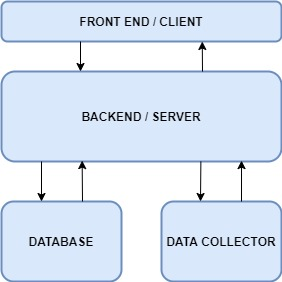
\includegraphics[width=0.4\textwidth]{images/ADS_overview.jpg}
 \caption{A simple architectural layer diagram}
\end{figure}

\subsection{Front-end Description}
%Each layer should be described separately in detail. Descriptions should include the features, functions, critical interfaces, and interactions of the layer. The description should clearly define the services that the layer provides. Also include any conventions that your team will use in describing the structure: naming conventions for layers, subsystems, modules, and data flows; interface specifications; how layers and subsystems are defined; etc. 
The front-end layer includes all software and hardware that is part of a product interface. The hardware includes PC, mobile phones, and tablets. The software is the code that is executed on the client-side (typically HTML, CSS, and JavaScript) that runs in the user's browser to create the user interface. Users interact directly with different components of the front-end, including user-entered data, buttons, links, and other features. The front-end includes subsystems such as login, register, shopping list, recipes, meal planning, and shop. The front-end is designed to be accessible, pleasant, and easy to use.

\subsection{Server Description}
The back-end layer is the code that runs on the server. The back-end receives requests from the front-end (client) and contains the logic of the application to process the request and return the appropriate data to the client. The back-end can directly interact with the database and data collector to retrieve the required data to fulfill the request. The back-end layer includes subsystems such as shopping manager, data parser, user management, query management, and database controller.

\subsection{Database Description}
The database layer stores and retrieves data. The database is also responsible for managing updates. The database layer includes multiple data tables that correspond with different functionalities of the product such as a table for a user, meal plan, shopping list, item, item-brand, brands, recipes, and recipe ingredients.
%Having a separate database layer will allow quick and flexible access to multiple concurrent requests from the webserver. Storing the data in a database also reduces the load on the main memory of the server CPU and provides security, data backup, ensuring the integrity of data, and access to data when the server crashes.

\subsection{Data Collector Description}
The data collector layer is responsible for retrieving data from multiple sources. There is one subsystem in the data collector layer, the API Manager. The data collector retrieves data from various stores through API and returns it to the backend layer.


\section{Roles \& Responsibilities}
Who are the stakeholders of the project? 
Software Developers & Customer & Profeesor
Who will be the point of contact from the sponsor or customer side? 
Tim Dockins
Who are the team members, and what will be their areas of responsibility? Will your team maintain the product owner and scrum master for the whole project, or will that role change periodically?
Uyen 
Kiran
Hozefa
Andrew
Patrick
We will most likeley maintain the product owner and the scrum master

This section should occupy 1/2 - 1 full page.
\section{Cost Proposal}
As this is a software project with no hardware component most of our expenses will be for licensing and hosting the application. We will be hosting the back-end of the application on Heroku's Free tier hosting but later on as the user base increases we would have to choose a different tier level which could add to our cost. We would also need to buy a domain name for the web application part of the project. The cost for these items should be covered by the senior design spending budget. 
 

\subsection{Preliminary Budget}
\begin{table}[h]
\centering

\begin{tabular}{|l|l|l|} 
\hline
Sr. No & Item               & Cost (\$)  \\ 
\hline
1.     & Heroku Hosting (Future)    & 200        \\ 
\hline
2.     & Domain Name (Future)        & 20         \\ 
\hline
3.     & API's (Future)             & 200        \\
\hline
 & \textbf{Total Cost}              & 420        \\
\hline
\end{tabular}\caption{Overview of the cost proposal}
\end{table}

\subsection{Current \& Pending Support}
The primary source of funding for this project is the default \$800 budget provided by the CSE depart-
ment for senior design teams. As this project is not sponsored, there is no external funding for the
project. There is no other support, expected or needed, pending.
\section{Facilities \& Equipment}
What lab space, testing grounds, makerspaces, etc. will you need to complete the project? Will you require any specific equipment, and if so, where will you get it (borrow, lease, purchase, outsource, already present in the lab, etc.). This section should occupy 1/2 page.
\section{Assumptions}
%An assumption is a belief of what you assume to be true in the future. You make assumptions based on your knowledge, experience or the information available on hand. These are anticipated events or circumstances that are expected to occur during your project's life cycle.
%
%Assumptions are supposed to be true but do not necessarily end up being true. Sometimes they may turn out to be false, which can affect your project significantly. They add risks to the project because they may or may not be true. For example, if you are working on an outdoor unmanned vehicle, are you assuming that testing space will be available when needed? Are you relying on an external team or contractor to provide a certain subsystem on time? If you are working at a customer facility or deploying on their computing infrastructure, are you assuming you will be granted physical access or network credentials?
%
%This section should contain a list of at least 5 of the most critical assumptions related to your project. For example:
%
%The following list contains critical assumptions related to the implementation and testing of the project.
%
Throughout the development lifecycle of this application, it is highly likely that many new issues and assumptions will arise.  
However, at present the following is a list of known assumptions for this application and its development process.

\begin{itemize}
  \item No members of the team will be lost.
  \item Time and schedule availability will persist for the duration of the project.
  \item The application will not have to be maintained after the final developmental increment.
  \item Developmental platforms will remain relatively constant.
  \item Regional and userbase scaling will not be a major issue during the lifetime of the application.
  \item Generally grocery stores will not have anything in their TOS preventing the use of scrapers on their websites.
  \item All users will have email addresses.
\end{itemize}
\section{Constraints}
%Constraints are limitations imposed on the project, such as the limitation of cost, schedule, or resources, and you have to work within the boundaries restricted by these constraints. All projects have constraints, which are defined and identified at the beginning of the project.
%
%Constraints are outside of your control. They are imposed upon you by your client, organization, government regulations, availability of resources, etc. Occasionally, identified constraints turn out to be false. This is often beneficial to the development team, since it removes items that could potentially affect progress.
%
%This section should contain a list of at least 5 of the most critical constraints related to your project. For example:
%
%The following list contains key constraints related to the implementation and testing of the project.
%
%
Consider the following list of developmental and deliverable constraints for this project.  This list is not exhaustive, but does contain the main identified constraints for this project.
\begin{itemize}
  \item Final prototype demonstration must be completed by April 21, 2022.
  \item Total development costs must not exceed \$800.
  \item Only stores which have been confirmed to allow scrapers or have affordable API's will be used within the app.
  \item Generally only major stores will be considered.
  \item The web-application should be compatible on mobile devices.
  \item Lists and such should be transferrable through the cloud.
  \item Users should be able to add their own recipes.
\end{itemize}

\section{Risks}
This section should contain a list of at least 5 of the most critical risks related to your project. Additionally, the probability of occurrence, size of loss, and risk exposure should be listed. For size of loss, express units as the number of days by which the project schedule would be delayed. For risk exposure, multiply the size of loss by the probability of occurrence to obtain the exposure in days. For example:

The following high-level risk census contains identified project risks with the highest exposure. Mitigation strategies will be discussed in future planning sessions.

\begin{table}[h]
\resizebox{\textwidth}{!}{
\begin{tabular}{|l|l|l|l|}
\hline
 \textbf{Risk description} & \textbf{Probability} & \textbf{Loss (days)} & \textbf{Exposure (days)} \\ \hline
 Availability of X sensor module due to contractor delay  & 0.50 & 20 & 10 \\ \hline
 Outdoor testing grounds are not available  & 0.20 & 14 & 2.8 \\ \hline
 Internet access not available at installation site  & 0.30 & 9 & 2.7 \\ \hline
 Delays in shipping from overseas vendors  & 0.10 & 20 & 2.0 \\ \hline
 Certification delays at compliance testing facility & 0.15 & 10 & 1.5 \\ \hline
\end{tabular}}
\caption{Overview of highest exposure project risks} 
\end{table}
\section{Documentation \& Reporting}
%%% In this section, you will describe all of the various artifacts that you will generate and maintain during the project life cycle. Describe the purpose of each item below, how the content will be generated, where it will be stored, how often it will be updated, etc. Replace the default text for each section with your own description. Reword this paragraph as appropriate.

\subsection{Major Documentation Deliverables}
%%% intentionally left blank
\subsubsection{Project Charter}
Version 1 of the Project Charter will be delivered on October 4, 2021 with Version 2 being delivered on December 6, 2021 and the final version being delivered on  April 29, 2022. The Project Charter will be reviewed every week during team meetings and will only be updated if four out of five team members agree on the update. The team will review and approve the Project Charter in the meeting that most immediately precedes the Charters due dates.

\subsubsection{System Requirements Specification}
Version 1 of the System Requirements Specification will be delivered on October 25, 2021 with Version 2 being delivered on December 6, 2021 and the final version being delivered on April 21, 2022. The System Requirements Specification will be reviewed every week during team meetings and will only be updated if four out of five team members agree on the update. The team will review and approve the System Requirements Specification in the meeting that most immediately precedes the System Requirements Specification due dates.

\subsubsection{Architectural Design Specification}
Version 1 of the Architectural Design Specification will be delivered on November 15, 2021 with Version 2 being delivered on December 6, 2021 and the final version being delivered on April 29, 2022. The Architectural Design Specification will be reviewed every week during team meetings and will only be updated if four out of five team members agree on the update. The team will review and approve the Architectural Design Specification in the meeting that most immediately precedes the Architectural Design Specification due dates.

\subsubsection{Detailed Design Specification}
Version 1 of the Detailed Design Specification will be delivered on February 22, 2022 and the final version being delivered on April 29, 2022. The Detailed Design Specification will be reviewed every week during team meetings and will only be updated if four out of five team members agree on the update. The team will review and approve the Detailed Design Specification in the meeting that most immediately precedes the Detailed Design Specification due dates.

\subsection{Recurring Sprint Items}
\subsubsection{Product Backlog}
Items will be added to the product backlog based on requirements from the customer and will only be done as a group. No members will be permitted to add items without the rest of the teams knowledge and approval. Priority will be given to backlog items based on the customer's input. All other items will then be given priority by the team through majority vote of four to one. The teams backlog will be maintained and accessible to all members via Jira. 

\subsubsection{Sprint Planning}
This project will have eight confirmed sprints with the possibility to add any during the winter break. All sprints will be planned by the team on the Fridays immediately preceding the beginning of the sprint. 

\subsubsection{Sprint Goal}
The customer will be given the option to set the team's sprint goal(s). In the case that the customer does not provide any, the sprint goal(s) will set by the team during the sprint planning meeting. These team set goals will be based on the priority of product backlog items and due dates of required documentation.

\subsubsection{Sprint Backlog}
The team's sprint backlog will be set before every sprint. The sprint backlog will be set based on the priority of items on the product backlog as well as estimated person hours needed to complete those items. The team will maintain the sprint backlog along with a scrum board via Jira.

\subsubsection{Task Breakdown}
Items from the sprint backlog will be assigned on Jira on a volunteer basis. This will allow for members to volunteer for items that would provide them an opportunity to learn something new while also creating the ability for team members to take on items they already know how to do when time becomes a bigger factor.

\subsubsection{Sprint Burn Down Charts}
The team manager will be responsible for the sprint burn down chart. The manager will use Jira to populate the burn down chart, but all members will be responsible for updating the progress of their assigned backlog items and logging the hours they put into completing those items. See Figure 1 for an example.

%\begin{figure}[h!]
%    \centering
%    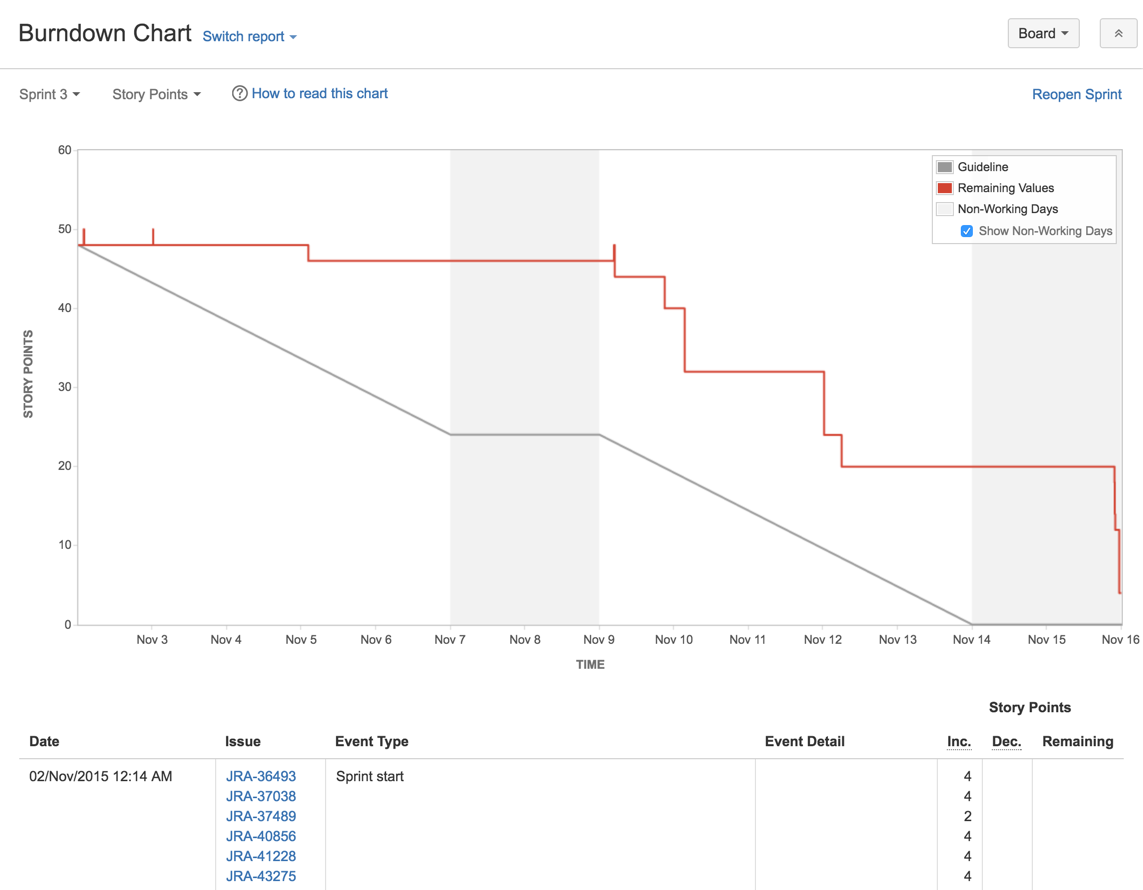
\includegraphics[width=0.5\textwidth]{images/burndown}
%    \caption{Example sprint burn down chart}
%\end{figure}
% \begin{center}
\begin{figure}
    \centering
    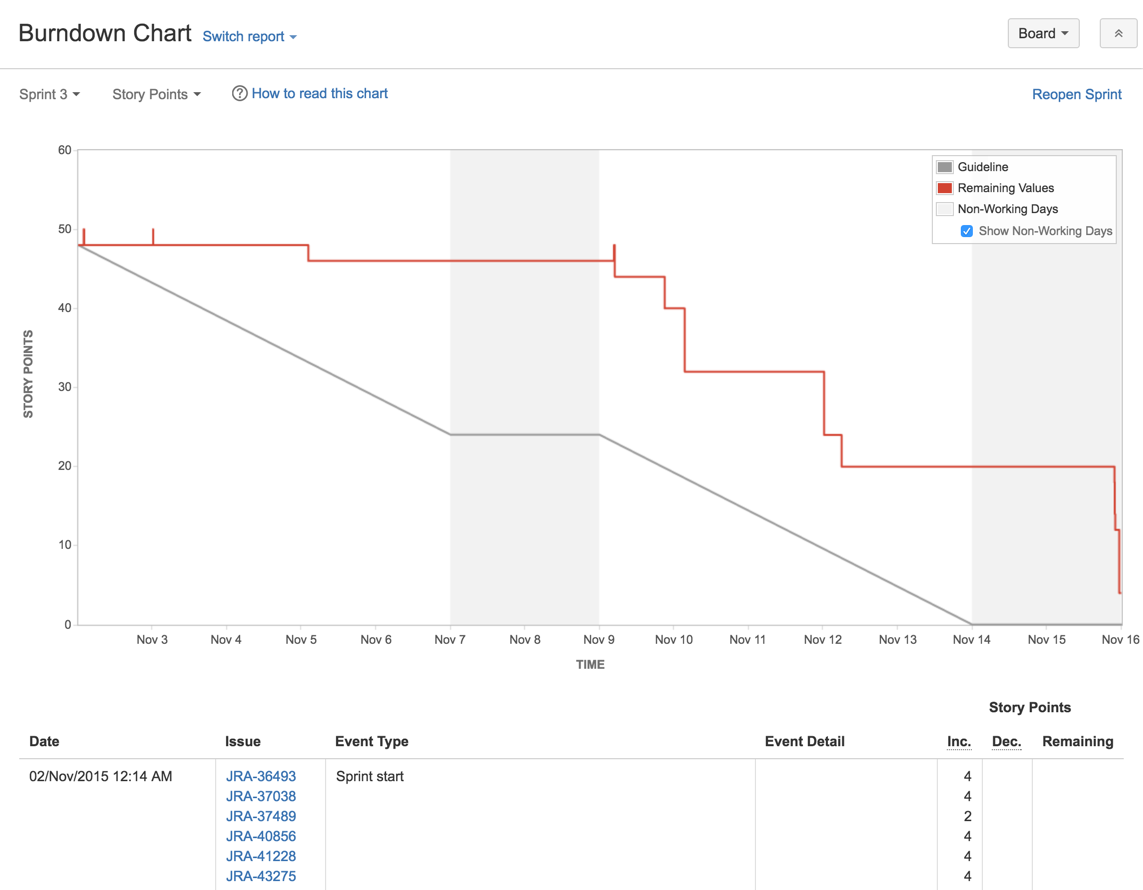
\includegraphics[width=0.5\textwidth]{images/burndown}\\
    \caption{Example sprint burn down chart}
\end{figure}
% \end{center}

\subsubsection{Sprint Retrospective}
The sprint retrospective will be created by all team members during the sprint review session that will take place during the Friday meetings at the end of each sprint. During these sprint review sessions, all team members will discuss the status of each sprint backlog items, the person hours put into them, and the team manager will populate the sprint burn down chart.

\subsubsection{Individual Status Reports}
Individual Status Reports are to be completed by each individual team member immediately following the end of sprints. Team members will use the sprint goal, sprint backlog, and sprint burn down chart that is agreed upon by the team. Team members will also use the sprint review session to help in the assessment of other team members. The sprint review session can also be used to create individual goals for the upcoming sprint. 

\subsubsection{Engineering Notebooks}
Each team member will be solely responsible for filling out their engineering notebook. Due to the setting of this project, all team members will disregard the witness signature for the engineering notebook.

\subsection{Closeout Materials}
\subsubsection{System Prototype}
The aim of this project is to meet all of the customer's requirements in the final system prototype. The final system prototype will first be demonstrated to the customer during the Prototype Acceptance Test. The final demonstration will take place on April 29, 2022.

\subsubsection{Project Poster}
The project poster will be delivered on April 29, 2022 during the final demonstration. The project poster will contain the system requirements, architectural design and design specifications and be 24" x 36". 

\subsubsection{Web Page}
The project web page will be hosted on the University's senior design project repository. The web page will be accessible to the public and be delivered on April 29, 2022. The web page will contain: the team name, the product name, the timeline that the team worked on the project, all team member's names, an abstract, background, project requirements, system overview, demo video, future plans and improvements for the project, and links to all documents and source code. 

\subsubsection{Demo Video}
The demo video is not required for this project anymore.

\subsubsection{Source Code}
All source code will be maintained in a private GitHub repository that will be accessible by all team members. Due to our customer's experience and knowledge of this project, they will have access to all source code upon request. This project will not be open sourced to the general public.

\subsubsection{Source Code Documentation}
Each team member will be responsible for properly documenting all code.

\subsubsection{Installation Scripts}
 In the case that this project is to be a desktop application, installation scripts will be provided to allow for the automatic installation for the customer.

\subsubsection{User Manual}
A short, easy to read user manual will be provided in the application that will be accessible to all users. The customer does not require any additional user manual documentation.

\newpage

%%% References
\bibliographystyle{plain}
\bibliographystyle{reference/IEEEtran_custom}
\bibliography{reference/refs}{}

\end{document}